\section{Исследование и построение решения задачи}\label{sec2}
\subsection{Восстановление снимков фМРТ по видеоряду}
Схема предлагаемого метода восстановления снимков фМРТ приведена на Рис.~\ref{fig:scheme}.

\begin{figure}[h!]
	\centering
	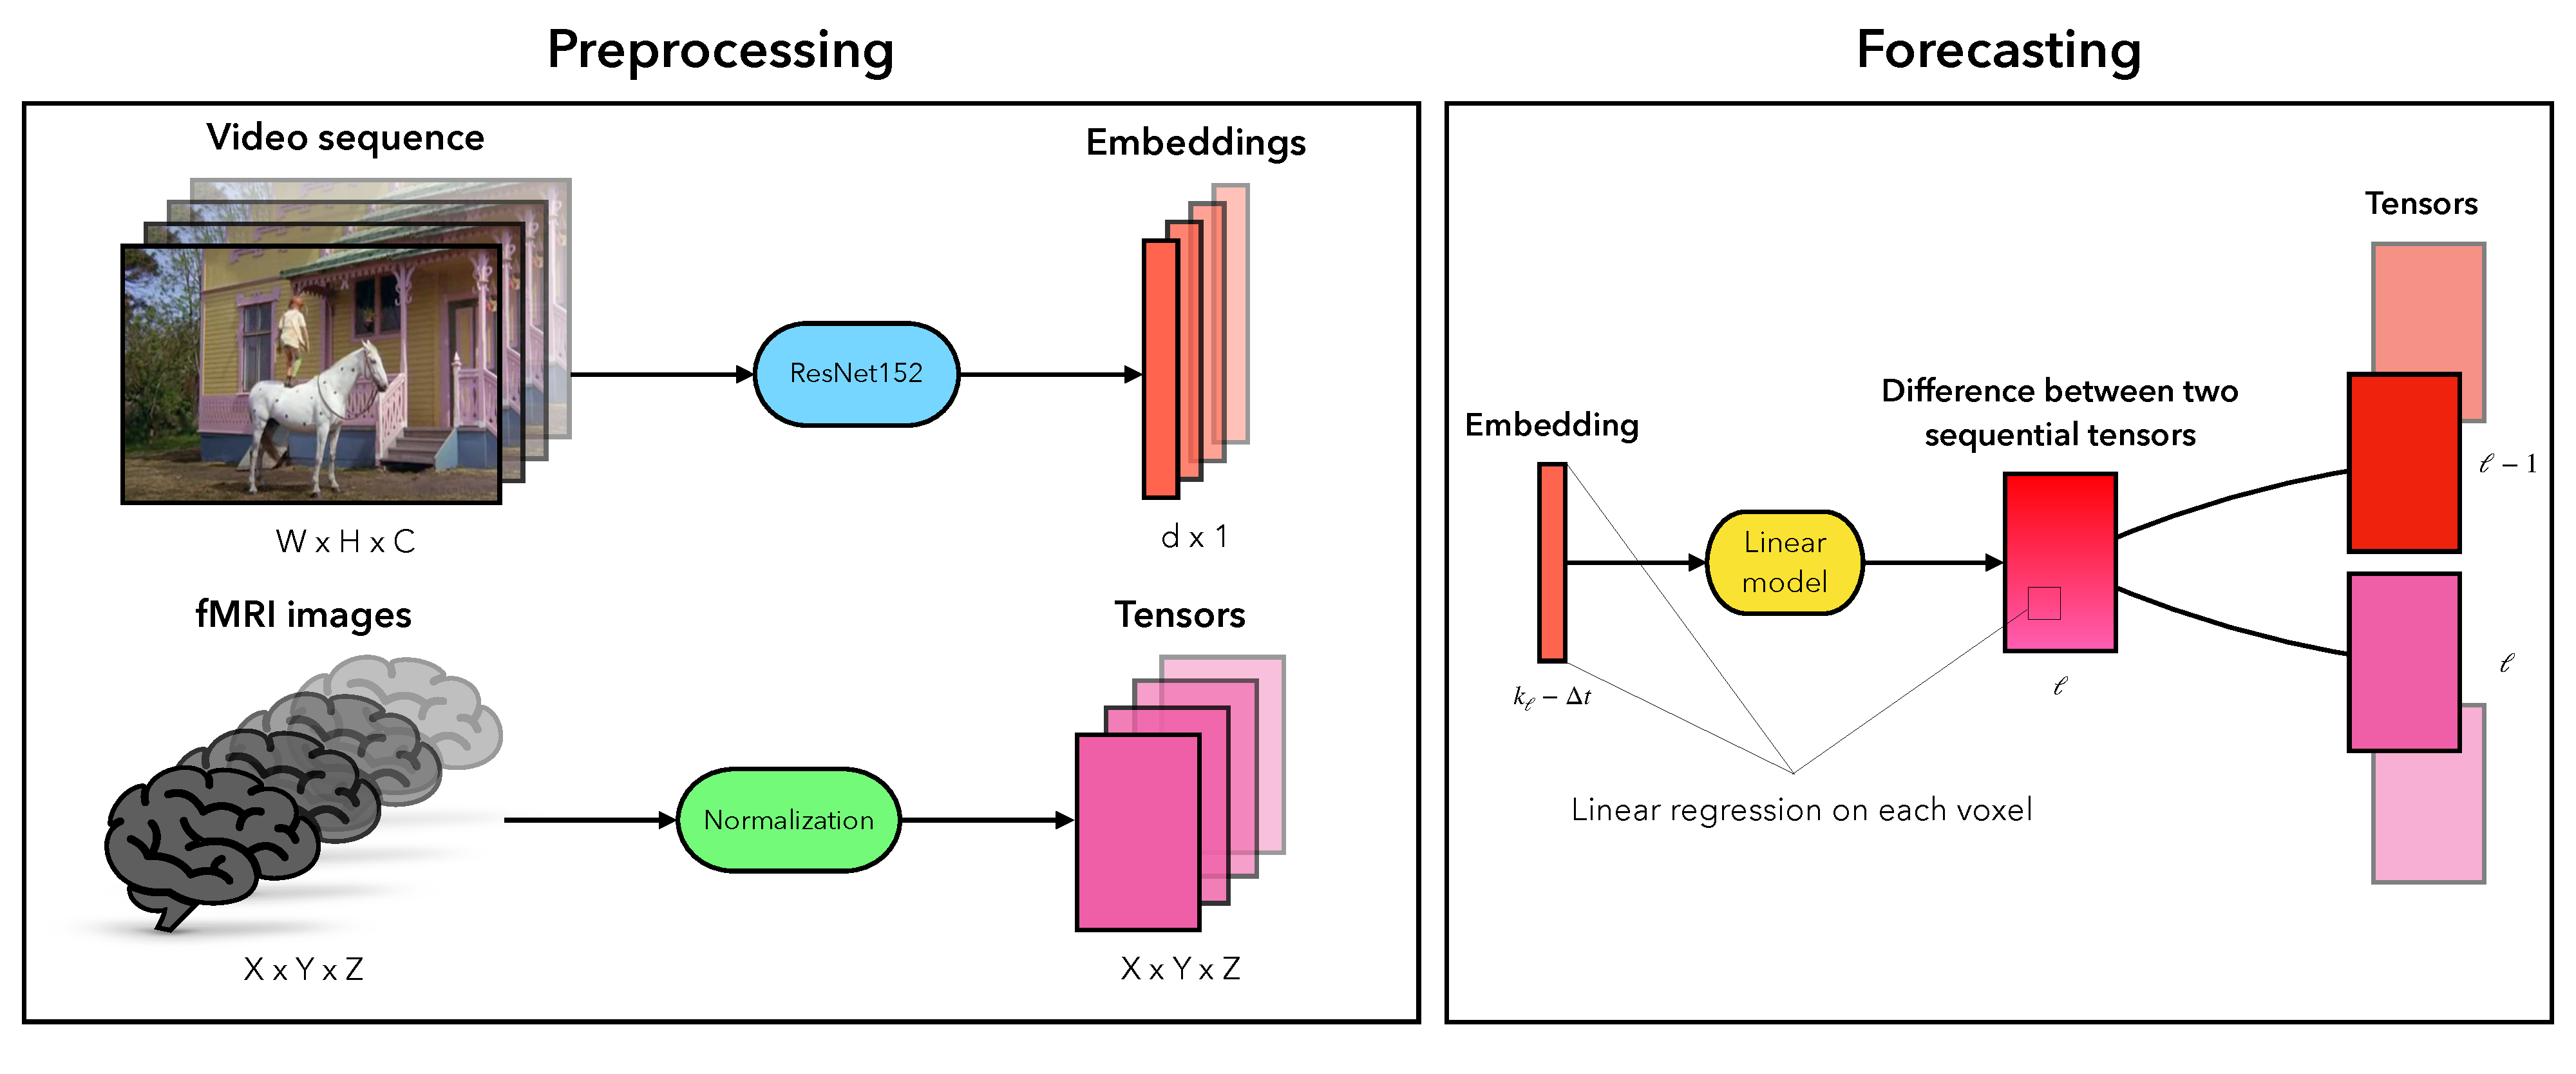
\includegraphics[width=1\textwidth]{images/scheme.pdf}
	\caption{Схема метода}
	\label{fig:scheme}
\end{figure}
Обозначим снимок фМРТ как $\bx_{\ell} = [v^{\ell}_{ijk}] \in \mathbb{R}^{X \times Y \times Z}$,
где $v^{\ell}_{ijk} \in \mathbb{R}_+$~--- значение соответствующего вокселя.
С целью сокращения времени работы метода предлагается использовать сжатие снимков фМРТ путем уменьшения размерностей.
Сжатие в 2 раза представляется в виде отображения
\[\bm{\chi}: \mathbb{R}^{X \times Y \times Z} \to \mathbb{R}^{X/2 \times Y/2 \times Z/2}.\]
Сжатие в $2^k$ раз получается применением $\bm{\chi}$ последовательно $k$ раз. 
Далее для простоты сохраняем обозначения размерностей снимков $X \times Y \times Z$.

Предположим, что для последовательности снимков выполнено марковское свойство,
т.е. каждый снимок зависит только от одного изображения и предыдущего снимка.
Тогда соответствующее отображение записывается в виде
\begin{equation*}
	\label{eq5}
	\mathbf{g}(\bp_{k_{\ell} - \nu \Delta t}) = \bx_{\ell} - \bx_{\ell-1} = \bdelta_{\ell}, \ \ell = 2, \ldots, \mu t.
\end{equation*}
где $\bdelta_{\ell} = [v^{\ell}_{ijk} - v^{\ell-1}_{ijk}] = [\delta^{\ell}_{ijk}] \in \mathbb{R}^{X \times Y \times Z}$~--- разность между двумя последовательными снимками.

Отображение $\mathbf{g}: \mathbf{P} \to \bX$ представляется в виде композиции
двух других:
\[ \mathbf{g} = \bm{\varphi} \circ \bm{\psi}, \]
\vspace{-0.8cm}
\begin{align*}
	 & \bm{\psi}: \mathbf{P} \to \mathbb{R}^d
	\text{~--- векторизация изображения,}        \\
	 & \bm{\varphi}: \mathbb{R}^d \to \bX
	\text{~--- восстанавливаемое отображение.}
\end{align*}

Для каждого изображения из видеоряда имеем вектор признакового описания размерности $d$:
\[ \bz_{\ell} = [z^{\ell}_1, \ldots, z^{\ell}_{d}]\T \in \mathbb{R}^{d}, \ {\ell} = 1, \ldots, \nu t. \]
Используется архитектура нейронной сети ResNet152 без последнего линейного слоя.

Учитывая \eqref{eq4}, суммарное число пар (изображение, снимок)
равно $N = \mu (t - \Delta t)$. Таким образом, для каждого вокселя задана выборка
\[ \mathfrak{D}_{ijk} = \{(\bz_{\ell}, \delta^{\ell}_{ijk}) \ | \ {\ell} = 2, \ldots, N \}. \]

Поставлена задача восстановления регрессии
\begin{equation*}
	\label{eq6}
	y_{ijk}: \mathbb{R}^{d} \to \mathbb{R}.
\end{equation*}

Используется линейная модель с вектором параметров
\[ \bw_{ijk} = [w^{ijk}_1, \ldots, w^{ijk}_{d}]\T \in \mathbb{R}^{d}: \]
\begin{equation*}
	\label{eq7}
	f_{ijk}(\bz, \bw_{ijk}) = \langle \bz, \bw_{ijk} \rangle.
\end{equation*}

Для модели $f_{ijk}$ с соответствующим ей вектором параметров $\bw_{ijk} \in \mathbb{R}^{d}$
определим квадратичную функцию потерь с $L_2$ регуляризацией:
\begin{equation*}
	\label{eq8}
	\mathcal{L}_{ijk}(\bw_{ijk}) = \sum\limits_{\ell = 2}^{N} \big(f_{ijk}(\bz_{\ell}, \bw_{ijk}) - \delta^{\ell}_{ijk}\big)^2 + \alpha \| \bw_{ijk} \|_2^2,
\end{equation*}
где $\alpha \in \mathbb{R}$~--- коэффициент регуляризации.

Требуется найти параметры, доставляющие минимум функционалу потерь $\mathcal{L}_{ijk}(\bw_{ijk})$
при заданных гиперпараметрах $\Delta t$ и $\alpha$:
\begin{equation*}
	\label{eq9}
	\hat{\bw}_{ijk} = \arg\min_{\bw_{ijk}} \mathcal{L}_{ijk}(\bw_{ijk}).
\end{equation*}

Минимум функции потерь находится методом наименьших квадратов. Определим матрицу объектов-признаков
\begin{equation*}
	\label{eq10}
	\bZ = [\bz_2, \ldots, \bz_N]\T = [z^i_j] \in \mathbb{R}^{(N-1) \times d}
\end{equation*}
и вектор, компонентами которого являются разности значений одного и того же вокселя в разных снимках,
\begin{equation*}
	\label{eq11}
	\mathbf{\Delta}_{ijk} = [\delta^2_{ijk}, \ldots, \delta^N_{ijk}]\T \in \mathbb{R}^{N-1}.
\end{equation*}

Решение записывается в виде
\begin{equation*}
	\label{eq12}
	\hat{\bw}_{ijk} = (\bZ\T \bZ + \alpha \mathbf{I})^{-1} \bZ\T \mathbf{\Delta}_{ijk}.
\end{equation*}

Получим формулу для восстановленных снимков фМРТ. Введем матрицу весов
\begin{equation*}
	\label{eq13}
	\hat{\bW} = [\hat{\bw}_1, \ldots, \hat{\bw}_{XYZ}]\T = [\hat{w}^i_j] \in \mathbb{R}^{XYZ \times d}.
\end{equation*}

Введем для тензоров $\bx_{\ell}, \bdelta_{\ell} \in \mathbb{R}^{X \times Y \times Z}$ векторы
\[ \bx_{\ell}^{R} = [ v^{\ell}_1, \ldots, v^{\ell}_{XYZ} ]\T,\
	\bdelta_{\ell}^{R} = [ \delta^{\ell}_1, \ldots, \delta^{\ell}_{XYZ} ]\T \in \mathbb{R}^{XYZ}. \]

Тогда вектор восстановленного снимка находится по формуле
\begin{equation*}
	\label{eq14}
	\hat{\bx}_{\ell}^{R} = \bx_{\ell-1}^{R} + \hat{\bdelta}_{\ell}^{R} = \bx_{\ell-1}^{R} + \hat{\mathbf{W}} \mathbf{z}_{\ell}.
\end{equation*}

\subsection{Классификация временных рядов фМРТ}
\subsubsection{Сегментация временного ряда фМРТ}\label{segmentation}
Имеется временной ряд фМРТ $\bX$ и соответствующий дискретный временной ряд стимулов $\bm{s}$:
\begin{equation*}
\bX = \left[\bx_{1}, \ldots, \bx_{T}\right], \quad \bx_{t} \in \mathbb{R}^{X \times Y \times Z},
\end{equation*}
\begin{equation*}
\bm{s} = \left[{s}_{1}, \ldots, {s}_{T}\right], \quad {s}_{t} \in \{0,\dots, C\},
\end{equation*}
где $X, Y$ и $Z$~--- размерности тензора снимка, $T$~--- длина временного ряда. 

Временной ряд стимулов $\bm{s}$ содержит информацию о том, какой стимул был представлен испытуемому в каждый момент времени $t$. Значения стимулов ${s}_{t}$ кодируются числами от $0$ до $C$. Кроме того, моменты отдыха испытуемого от стимула обозначены как $s_t = 0$.
\begin{assumption}
    В работе предполагается, что испытуемый имел достаточное время для отдыха между демонстрацией стимулов разных категорий. На практике, данное предположение обычно выполняется, что позволяет избежать пересечения эффектов от различных стимулов. 
\end{assumption}
Построим сегментацию $\mathcal{G}(\bX, \bm{s})$ временного ряда $\bX$.
Для каждой категории $k \in \{1,\dots,C\}$ выделим из временного ряда $\bX$ сегменты фиксированной длины $\tau$ следующим образом:
\begin{enumerate}
	\item Находим индексы начала и конца отрезков, соответствующих классу стимула $k$. 
	Обозначим индексы в порядке возрастания $\{b_{1}, \ldots, b_{n_{k}}\}$ и $\{e_{1}, \ldots, e_{n_{k}}\}$ соответственно, 
	где $n_{k}$~--- число отрезков, отвечающих категории $k$. 
	Формально данные индексы определяются как:
	\begin{equation*}
	\{b_{1}, \ldots, b_{n_{k}}\} = \{t \mid {s}_{t}=k, {s}_{t-1}=0\},
	\end{equation*}
	\begin{equation*}
	\{e_{1}, \ldots, e_{n_{k}}\} = \{t \mid {s}_{t}=k, {s}_{t+1}=0\},
	\end{equation*}

	\item Для каждого сегмента $[b_{j},~e_{j}] \subset [1,~T]$ длины $\tau_{j} = e_{j} - b_{j} + 1$ добавим слева и 
	справа сегменты, отвечающие моментам отдыха испытуемого,  
	чтобы получить отрезок длины $\tau$:
	\begin{equation*}
	\bX_{j} = [\bx_{b_{j}-\delta_1}, \ldots, \bx_{e_{j}+\delta_2}],
	\end{equation*}
	\begin{equation*}
		\bm{s}_{j} = [s_{b_{j}-\delta_1}, \ldots, s_{e_{j}+\delta_2}],
	\end{equation*}
	где $j = 1,\ldots, n_{k}, \quad \delta_1 = \lfloor (\tau - \tau_{j})/2 \rfloor$, $\delta_2 = \lceil (\tau - \tau_{j})/2 \rceil$. Здесь $\lfloor \cdot \rfloor$ и $\lceil \cdot \rceil$ обозначают операции округления в меньшую и большую сторону соответственно.
        
	Обратим внимание, что для каждой категории $k$ предполагается $\tau_{j} < \tau,\quad j = 1,\ldots, n_{k}$.

	\item В результате объединения по всем категориям получим $N = \sum_{k=1}^C n_k$ сегментов временного ряда длины $\tau$. Формально получаем:
	\begin{equation*} 
		\bX = \{\bX_1,\dots, \bX_{N}\},
	\end{equation*}
	\begin{equation*}
		\bX_j = [\bx_{1}^j, \ldots, \bx_{\tau}^j], \quad
		\bx_{t}^j \in \mathbb{R}^{X \times Y \times Z},
	\end{equation*}
	$$\bm{s}_j = \left[s_1^j, \dots, s_{\tau}^j\right], \quad s_t \in \{0,~1\},$$
	$$\bm{y} = \left[y_1, \dots, y_{N}\right],\quad y_j \in \{1,\dots, C\},$$
	где $y_j$~--- метка класса временного ряда $\bX_j$, $\bm{s}_j$~--- временной ряд стимулов, где $s_t^j$ принимает ненулевое значение в моменты стимулирования категории $y_j$.
\end{enumerate}


\subsubsection{Взвешивание вокселей фМРТ снимков}
Предлагается метод \textit{Cross-Correlation Weighting} взвешивания активных областей мозга в задаче декодирования временных рядов фМРТ. Результатом работы алгоритма является бинарная маска $\mathcal{M} \in  \mathbb{R}^{X \times Y \times Z}$, в которой ненулевым значениям соответствуют области человеческого мозга, реагирующие на стимул.

Имеется временной ряд фМРТ $\bX$ и соответствующий дискретный временной ряд стимулов $\bm{s}$:
\begin{equation*}
\bX = \left[\bx_{1}, \ldots, \bx_{\tau}\right], \quad \bx_{t} \in \mathbb{R}^{X \times Y \times Z},
\end{equation*}
\begin{equation*}
\bm{s} = \left[{s}_{1}, \ldots, {s}_{\tau}\right], \quad {s}_{t} \in \{0,~1\},
\end{equation*}
где $X, Y$ и $Z$~--- размерности тензора снимка, $T$~--- длина временного ряда. Временной ряд стимулов $\bm{s}$ содержит информацию о моментах стимулирования испытуемого. Моменты отдыха от стимула обозначены как $s_t = 0$, в то время как моменты стимулирования~--- $s_t = 1$. Обратим внимание, что предполагается однотипное стимулирование в ходе испытания.
\begin{assumption}
        Наличие неизменяющегося времени гемодинамической ответной реакции зависимости уровня кислорода в крови.
     \end{assumption}
        \begin{assumption}
        Если область мозга реагирует на стимул, то значение кросс-корреляционной функции для вокселей из этой области ожидается большим.
    \end{assumption}

Предложенный метод состоит из следующих этапов:
\begin{enumerate}
    \item На вход подается временной ряд фМРТ $\bX$ с частотой снимков $\mu$ и временной ряд стимулов $\bm{s}$.
    \item 3D Average Pooling: ко всем изображениям фМРТ в $\bX$ применяется свертка $\textbf{AvgPool3d}(~\cdot~,  k_s)$ с ядром $k_s$:

    \begin{equation*}
    \bX' = \left[\bx'_1, \dots, \bx'_{\tau}\right],
    \end{equation*}
    \begin{equation*}
    \bx'_t = \textbf{AvgPool3d}(\bx_t, k_s) \in \mathbb{R}^{X/ k_s \times Y/ k_s \times Z/ k_s}, 
    \end{equation*}
    где $\bX'$~--- это сжатые данные фМРТ.
    \item Z-нормализация временных рядов: временные ряды каждого вокселя в сжатых данных фМРТ $\bX'$ нормализуются путем вычитания их выборочного среднего и деления на несмещенную оценку стандартного отклонения. 
	Аналогично нормализуется временной ряд $\bm{s}$. 
	Обозначим нормализованные данные $\hat{\mathbf{\bX'}}$ и $\hat{\bm{\bm{s}}}$ соответственно. 


    \item Вычисление кросс-корреляции: введем обозначение $v^{i,j,k}_t$~--- значение вокселя снимка фМРТ $\hat{\mathbf{\bx'}}_t$ в позиции $(i,~j,~k)$. Тогда для каждой тройки индексов $(i,~j,~k)$ определим функцию кросс-корреляции между временным рядом вокселя $\bm{v}^{i,j,k}$ и временным рядом стимулов $\hat{\bm{\bm{s}}}$ следующим образом:
    
    \begin{equation*}
        c_{i,j,k}\left(p\right) = \left(\hat{\bm{\bm{s}}} * \bm{v}^{i,j,k}\right)\left(p\right)=\dfrac{1}{\tau-1}\sum_{t=1}^{\tau-p} \hat{s}_{t} \cdot v^{i,j,k}_{t+p}, \quad p = 0, \ldots, \tau-1,\quad \text{где}
    \end{equation*}
        $$\bm{v}^{i,j,k}=\left[v^{i,j,k}_1, \dots v^{i,j,k}_{\tau}\right],$$
        $$\hat{\bm{\bm{s}}} = \left[\hat{s}_1, \dots \hat{s}_{\tau}\right].$$ 


    \item Воспользуемся предположениями.
    Формально есть задержка $\Delta t$, которая является параметром метода. Вычислим дискретный момент времени соответствующий задержке:
    $$p_{\Delta t} = \lfloor\mu\Delta t \rfloor.$$
    Находим значение кросс-корреляционной функции $c_{i,j,k}(p_{\Delta t})$ для каждой тройки индексов $(i,~j,~k)$. 
	Рассмотрим нулевой тензор $\mathcal{M}_c \in \mathbb{R}^{X/ k_s \times Y/ k_s \times Z/ k_s}$.
 
	Теперь присваиваем единицы для значений тензора в позициях $(i,~j,~k)$, соответствующих $h$ наибольшим значениям $c_{i,j,k}(p_{\Delta t})$. В итоге получаем маску, однако сжатую.

	\item В завершение процедуры выполняем операцию обратной свертки, также известную как upsample, которая позволяет получить тензор $\mathcal{M}$ с разрешением $X \times Y \times Z$.

    В этой операции назначаем каждому элементу тензора $\mathcal{M}_c$ с разрешением $X/ k_s \times Y/ k_s \times Z/ k_s$ маленький тензор размером $k_c \times k_c \times k_c$. Значения этого маленького тензора совпадают со значениями элемента в $\mathcal{M}_c$.
	
\end{enumerate}
Метод имеет три настраиваемых параметра: размер ядра $k_c$, время гемодинамической ответной реакции 
$\Delta t$ и число активных областей $h$.

\paragraph*{Статистический анализ локализованных областей мозга.}
\phantomsection % Создаем невидимую ссылку
\label{par:stat_anal} % Ставим метку с именем "par:stat_anal"
Для проверки статистической значимости областей, полученных с помощью метода \textit{Cross-Correlation Weighting}, предлагается проверить значимость корреляции между временным рядом стимула и временным рядом каждого вокселя фМРТ. Воспользуемся выборочным коэффициентом корреляции Кенделла. 
\begin{definition}
Выборочный коэффициент корреляции Кендалла:
$$\hat{\tau}_{X_1X_2} = 1 - \frac{4}{n\left(n-1\right)} \sum_{i=1}^{n-1} \sum_{j=1}^n \left[\left[X_{1i}<X_{1j}\right]\neq\left[X_{2i}<X_{2j}\right]\right] = \frac{C-D}{C+D},$$
где $X_1,~X_2$~--- выборки объема $n$, $C$~--- число согласованных пар, $D$~--- число несогласованных пар.
\end{definition}
Рассмотрим временной ряд $\bm{v}$ каждого вокселя фМРТ и временной ряд стимула $\bm{s}$, тогда применим следующий критерий:
\begin{center}
			\begin{tabular}{rl}
				выборки:                        & $\bm{v}=\left[v_{1},\ldots,v_{\tau}\right]$\\
				                                & $\bm{s}=\left[s_{1},\ldots,s_{\tau}\right]$\\
				                                & выборки связанные\\
				нулевая гипотеза:               & $H_0\colon \tau_{\bm{v}\bm{s}}=0$ \\
				альтернатива:                   & $H_1\colon \tau_{\bm{v}\bm{s}}>0$ \\
				статистика:                     & $\hat{\tau}_{\bm{v}\bm{s}}$ \\
				нулевое распределение:          & табличное\\
			\end{tabular}
		\end{center}
При справедливости $H_0$:
$$\mathbb{E}\hat{\tau}_{\bm{v}\bm{s}} = 0, \;\; \mathbb{D}\hat{\tau}_{\bm{v}\bm{s}} = \frac{2\left(2\tau+5\right)}{9\tau\left(\tau-1\right)}.$$
Ставится задача множественного тестирования гипотез, так как критерий применяется для каждого вокселя фМРТ. Делаем поправку Холма на множественное тестирование гипотез. Последним шагом отбираем позиции вокселей, где гипотеза с учетом поправки отвергается. Корреляция полученных областей мозга со стимулом статистически значима. 

\subsubsection{Классификация сегментов временного ряда фМРТ}
Схема предлагаемого метода классификация сегментов временного ряда фМРТ приведена на Рис.~\ref{fig:scheme_2}.
\begin{figure}[h!]
	\centering
	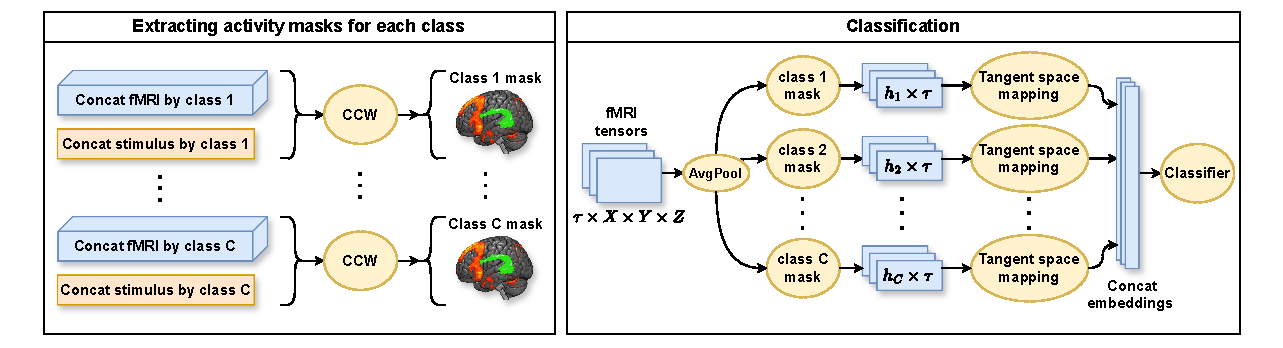
\includegraphics[width=1\textwidth]{images/scheme_2.pdf}
	\caption{Схема метода}
	\label{fig:scheme_2}
\end{figure}

Пусть имеется $N$ сегментов временного ряда фМРТ длины $\tau$. Кроме того, имеются временные ряды стимулов и метки классов, соответствующие сегментам. Формально:
	\begin{equation*} 
		\bX = \{\bX_1,\dots, \bX_{N}\},
	\end{equation*}
	\begin{equation*}
		\bX_j = [\bx_{1}^j, \ldots, \bx_{\tau}^j], \quad
		\bx_{t}^j \in \mathbb{R}^{X \times Y \times Z},
	\end{equation*}
	$$\bm{s}_j = \left[s_1^j, \dots, s_{\tau}^j\right], \quad s_t \in \{0,~1\},$$
	$$\bm{y} = \left[y_1, \dots, y_{N}\right],\quad y_j \in \{1,\dots, C\},$$
	где $y_j$~--- метка класса временного ряда $\bX_j$, $\bm{s}_j$~--- временной ряд стимулов, где $s_t^j$ принимает ненулевое значение в моменты стимулирования категории $y_j$.
 \paragraph*{Извлечение масок активности мозга для каждой категории стимула.}
Задана обучающая выборка:
\[ \mathfrak{D} = \{(\bX_{j}, \bm{s}_j, y_j) \ | \ {j} = 1, \ldots, N \}. \]
Выделение маски активности мозга для каждой категории стимула позволяет выделить специфичные для каждого класса области мозга, которые активируются в ответ на соответствующий стимул.

Без ограничения общности рассмотрим произвольный класс $k \in \{1, \ldots, C\}$. Выделим подвыборку $\mathfrak{D}_k$, соответствующую классу $k$, и перенумеруем для удобства объекты подвыборки:
\[\mathfrak{D}_k = \{(\bX_j, \bm{s_j}, y_j) \in \mathfrak{D}\ | \ y_j = k\} = \{(\bX_j, \bm{s_j})\ | \ j = 1,\ldots, N_k\}.\]
При использовании метода \textit{Cross-Correlation Weighting} на отдельном объекте подвыборки нет гарантии, что полученная маска соответствует нужной области мозга, отвечающей стимулированию класса $k$. Это связано в первую очередь с ограничениями и недостатками процедуры фМРТ, о чем подробно написано в разделе \ref{intro} Поэтому для повышения статистической значимости анализа предлагается брать усредненную активность по объектам подвыборки. Для этого рассмотрим конкатенацию временных рядов фМРТ и стимула вдоль временной координаты. Формально для подвыборки $\mathfrak{D}_k$ получаем:
\[
\bX^k = \bX_1 \oplus \bX_2 \oplus \ldots \oplus \bX_{N_k},
\]
\[
\bm{s}^k = \bm{s}_1 \oplus \bm{s}_2 \oplus \ldots \oplus \bm{s}_{N_k},
\]
\[\bX^k \in \mathbb{R}^{\tau N_k \times X \times Y \times Z}, \quad \bm{s}^k \in \{0, 1\}^{\tau N_k},\]
где операция $(~\cdot~\oplus~\cdot~)$~--- конкатенация по первой координате.
К полученным рядам $\bX^k$ и $\bm{s}^k$  применяем метод \textit{Cross-Correlation Weighting} с гиперпараметрами $h_k,~k_s$, считаем, что задержка учтена $\Delta t$ = 0. Решено не делать шаг с Upsample, так как применение Average Pooling к тензорам фМРТ позволяет уменьшить влияние аномальных или шумовых вокселей на анализ активности головного мозга. Получаем для категории стимула $k$ сжатую бинарную маску активности $\mathcal{M}^k \in \{0, 1\}^{X/k_s\times Y/k_s \times Z/k_s}$. 
\begin{definition}\label{def:def6}
Формально определим операцию применения бинарной маски активности к временному ряду фМРТ.
Пусть задан временной ряд фМРТ: 
$$\bX = [\bx_{1}, \ldots, \bx_{\tau}], \quad \mathbf{x}_{t} \in \mathbb{R}^{X \times Y \times Z}.$$
Задана бинарная маска активности головного мозга:
\[\mathcal{M} \in \{0, 1\}^{X \times Y \times Z}.\]
Если в вокселе $(i,~j,~k)$ присутствует активность, то $\mathcal{M}(i,~j,~k) = 1$, иначе $\mathcal{M}(i,~j,~k) = 0$.
Тогда операция применения маски $\mathcal{M}$ к временному ряду $\mathbf{X}$ определяется как:
$$\mathbf{Z} = \mathcal{M} \bullet \mathbf{X} = [\bz_{1}, \ldots, \bz_{\tau}],$$
где $\bz_{t} \in \mathbb{R}^{h}$, $h$~--- число ненулевых элементов в маске $\mathcal{M}$.
$$\bz_{t}(\ell) = \bx_{t}(i,~j,~k), \quad \text{где} \quad (i,~j,~k) = \mathrm{ind}_{\ell}(\mathcal{M}).$$
$\mathrm{ind}_{\ell}(\mathcal{M})$~--- функция, возвращающая индексы $\ell$-го ненулевого вокселя в маске $\mathcal{M}$.
В результате операции применения маски получаем матрицу $\bZ \in \mathbb{R}^{h\times \tau}$.
\end{definition}

\paragraph*{Классификация сегментов временного ряда.}
Задана обучающая выборка:
\[ \mathfrak{D} = \{(\bX_{j}, y_j),~\bX_{j}\in \mathbb{R}^{\tau\times X\times Y \times Z} \ | \ {j} = 1, \ldots, N \}. \]
Кроме того, для каждой категории стимулов задана сжатая с ядром $k_s$ бинарная маска активности:
\[\bm{M} = \{\mathcal{M}^k \in \{0, 1\}^{X/k_s\times Y/k_s \times Z/k_s}\ | \ k = 1, \ldots, C\}.\]
Искомое отображение $g: \bX \rightarrow \{1,\ldots, C\}$ представляется в виде композиции трех других:
\[g \coloneqq \bm{\varphi} \circ \bm{\psi} \circ \mathcal{A}, \]
\vspace{-0.8cm}
\begin{align*}
        & \mathcal{A}: \bX \to \mathbb{R}^{\tau \times X/k_s \times Y/k_s \times Z/k_s}
	\text{~--- Average Pooling,}        \\
	 & \bm{\psi}: \mathbb{R}^{\tau \times X/k_s \times Y/k_s \times Z/k_s} \to \mathbb{R}^d
	\text{~--- векторизатор,}        \\
	 & \bm{\varphi}: \mathbb{R}^d \to \{1,\ldots, C\}
	\text{~--- классификатор.}
\end{align*}
Отображение $\mathcal{A}$~--- применение 3d Average Pooling с ядром $k_s$ к каждому тензору фМРТ во временном ряду.

Построим отображение $\bm{\psi}$ и определим размерность эмбеддингов $d$. Обозначим число ненулевых элементов в $\mathcal{M}^k$ как $h_k,~k = 1, \ldots, C$. Отображение $\bm{\psi}$ является конкатенацией отображений $\bm{\psi}_k,~k = 1, \ldots, C$. Запишем формально:
\[\bm{\psi} \coloneqq \bm{\psi}_1 \oplus \ldots \oplus \bm{\psi}_C,\]
\[
\bm{\psi}_k: \bX \rightarrow \mathbb{R}^{d_k}, \quad k = 1, \ldots, C,
\]
\[d = \sum_{k=1}^C d_k.\]
Для каждой категории $k \in \{1, \ldots, C\}$ отображение $\bm{\psi}_k$ представимо в виде композиции двух отображений:
\[\bm{\psi}_k \coloneqq \bm{\pi}_k \circ \bm{f}_k.\]
Здесь $\bm{f}_k:\mathbb{R}^{\tau \times X/k_s \times Y/k_s \times Z/k_s} \rightarrow \mathbb{R}^{h_k\times \tau}$~--- применение маски активности $\mathcal{M}^k$, см. 
\hyperref[def:def6]{Определение 6}.
Отображение $\bm{\pi}_k: \mathbb{R}^{h_k\times \tau} \rightarrow \mathbb{R}^{d_k}$~--- проекция на риманово касательное пространство с последующей векторизацией.

Подробнее остановимся на методе $\bm{\pi}_k$ трансформации признакового пространства в терминах римановой геометрии \citep{barachant2010riemannian, barachant2011multiclass}. В работе \citep{barachant2011multiclass} метод называется \textit{Tangent Space Mapping}.
Первым шагом данного алгоритма является формирование пространства центрированных признаков. Введем следующие обозначения: 
$$\bY^k_j = \accentset{\circ}{\bm{f}_k(\mathcal{A}(\bX}_j)), \quad j = 1, \ldots, N,$$

\begin{equation*}
	\bY^k_j= \left[
\begin{array}{cccc}
y^{kj}_{11} & y^{kj}_{12} & \ldots & y^{kj}_{1\tau}\\
y^{kj}_{21} & y^{kj}_{22} & \ldots & y^{kj}_{2\tau}\\
\vdots & \vdots & \ddots & \vdots\\
y^{kj}_{h_k1} & y^{kj}_{h_k 2} & \ldots & y^{kj}_{h_k\tau}
\end{array}
\right]
	= \begin{bmatrix}
		\bm{y}^{kj}_1\\
            \bm{y}^{kj}_2\\
		\vdots\\
		\bm{y}^{kj}_{h_k}
		\end{bmatrix},\quad j = 1, \ldots, N,
	\end{equation*}
где $\bm{y}^{kj}_i, \quad i = 1, \ldots, h_k$~--- центрированные временные ряды.
Тогда ковариационная матрица для $\bY^k_j$~--- многомерного временного ряда:
$$ \bm{R}^k_j = \dfrac{1}{\tau-1}{\bY^k_j\bY^k_j}^{\T}, \quad \bm{R}^k_j \in \mathbb{R}^{h_k\times h_k}, \quad j = 1, \ldots, N.$$

Известно, что пространство, состоящее из матриц ковариации, представляет собой 
Риманово многообразие \citep{barachant2010riemannian}. 
В каждой точке риманова многообразия имеется касательная плоскость с 
определенным на ней скалярным произведением. Общая касательная плоскость для проекции матриц ковариации в выборке формируется в точке среднего геометрического по римановой метрике 
известных ковариационных матриц. Среднее геометрическое симметричных положительно определенных матриц \citep{moakher2005differential} имеет вид:
$$\bm{R}_k = \mathfrak{G}\left(\bm{R}^k_1,\dots,\bm{R}^k_N\right) = \underset{\bm{R}}{\arg \min}\sum_{j = 1}^N
\delta^2_R(\bm{R},~\bm{R}^k_j),$$
где риманова метрика или геодезическое расстояние определяется следующим образом:
$$\delta_R(\bm{R}_1,~\bm{R}_2) = \|\log (\bm{R}_1^{-1}\bm{R}_2)\|_F = \sqrt{\sum_{i = 1}^{3N} \log^2\lambda_i}.$$
Здесь $\lambda_i$~--- собственные значения матрицы $\bm{R}_1^{-1}\bm{R}_2$. В работе \citep{barachant2010riemannian}
получено, что для каждой ковариационной матрицы $\bm{R}^k_j$ существует проекция $\bm{\pi}^k_j$ на касательное пространство.
Кроме того, определено отображение:
$$\text{Exp}_{R}(\bm{\pi}^k_j) = \bm{R}^k_j = \bm{R}_k^{\frac{1}{2}} \exp\left(\bm{R}_k^{-\frac{1}{2}}\bm{\pi}^k_j\bm{R}_k^{-\frac{1}{2}}\right) \bm{R}_k^{\frac{1}{2}}$$
$$\text{Log}_{R}(\bm{R}^k_j) = \bm{\pi}^k_j = \bm{R}_k^{\frac{1}{2}} \log\left(\bm{R}_k^{-\frac{1}{2}}\bm{R}^k_j\bm{R}_k^{-\frac{1}{2}}\right) \bm{R}_k^{\frac{1}{2}}$$
После проектирования каждой ковариационной матрицы $\bm{R}^k_j$ с помощью $\text{Log}_{R}(~\cdot~)$, получаем
матрицы $\bm{\pi}^k_j \in \mathbb{R}^{h_k\times h_k}$. 
Последним шагом метода является векторизация.
Процесс векторизации каждой матрицы $\bm{\pi}^k_j$ в пространство с евклидовой метрикой~---
последовательная запись элементов верхнетреугольной матрицы от $\bm{\pi}^k_j$, 
где диагональные элементы имеют коэффициент 1, а недиагональные~--- коэффициент $\sqrt{2}$. 
Получаем эмбеддинги:
\begin{equation*}
	\hat{\bm{\pi}}^k_j = \begin{bmatrix}
		\bm{\bm{\pi}}^k_j({1,~1}) & \sqrt{2} \bm{\pi}^k_j({1,~2}) &  \ldots  &  \sqrt{2}\bm{\pi}^k_j(1,~h_k) & \bm{\pi}^k_j({2,~2}) & \ldots & \bm{\pi}^k_j({h_k,~h_k})
		\end{bmatrix}^{\T},
\end{equation*}
\[\hat{\bm{\pi}}^k_j \in \mathbb{R}^{d_k},\quad d_k = \dfrac{h_k(h_k+1)}{2}.\]
Важно подчеркнуть, что при таком подходе извлекаются пространственные характеристики, которые демонстрируют степень соответствия объекта маске активности конкретного класса.

В качестве классификатора $\bm{\varphi}$ рассматриваются традиционные варианты, такие как логистическая регрессия и перцептрон с двумя скрытыми слоями.
\newpage
